\documentclass[lettersize,journal]{IEEEtran}

\usepackage{amsmath,amsfonts,amssymb}
\usepackage{algorithm}
\usepackage{algorithmic}
\usepackage{array}
\usepackage{booktabs}
\usepackage{multirow}
\usepackage{textcomp}
\usepackage{stfloats}
\usepackage{url}
\usepackage{graphicx}
\usepackage{cite}
\usepackage{xcolor}

\hyphenation{MATPOWER Pyomo Egret ProOPF post-training}

% Visible notes are intentional in this first full-paper draft.  Remove them
% only after the corresponding experiment, reference, or author decision is
% complete.
\newcommand{\drafttodo}[1]{\textcolor{red}{\textbf{[TODO: #1]}}}
\newcommand{\methodname}{Power-Reward}
\newcommand{\dataset}{ProOPF-DP-v11}
\newcommand{\benchmark}{ProOPF-BP-v6}

\begin{document}

\title{Physics-Aware and Execution-Verifiable Post-Training for Language-Driven Optimal Power Flow Model Adaptation}

\author{Yifan Zhang and Coauthors to Be Confirmed%
\thanks{Y. Zhang is with the School of Advanced Manufacturing and Robotics, Peking University, Beijing, China (e-mail: 2601112747@stu.pku.edu.cn).}%
\thanks{The complete author list, author order, corresponding author, affiliations, and funding statement are to be confirmed before submission.}}

\maketitle

\begin{abstract}
Power-system studies repeatedly adapt optimal power flow (OPF) models to updated forecasts, equipment availability, operating limits, and security or policy requirements. A large language model (LLM) can assist this process, but regenerating a complete OPF program is both unnecessary and error-prone: syntactically valid code may modify the wrong grid object, perform a silent no-op, or create a constraint that is never attached to the optimization model. This paper formulates language-driven OPF modeling as a constrained model-adaptation task. A validated Python/Egret backbone remains fixed, while the LLM produces a machine-readable specification, a parameter-modification hook, and a structural-extension hook. We construct 4,400 training and development examples and a separately rebuilt 123-task benchmark covering explicit and scenario-inferred parameter changes with and without structural extensions. All records pass parameter-target and post-state auditing, while the structural verifier is validated across nine extension families and targeted counterexamples. A cumulative curriculum teaches the four adaptation capabilities, and we propose a three-stage Physics-Aware \methodname{} that combines interface validity, realized grid/model correctness, and execution/solver feedback. The deterministic components currently support data auditing and strict candidate evaluation and are designed for integration into the final reinforcement-learning reward. Preliminary experiments on the pre-freeze data version show that supervised fine-tuning substantially improves executable generation, especially with demonstrations. \drafttodo{Replace the preliminary statement with final \dataset{}/\benchmark{} SFT and RL results.}
\end{abstract}

\begin{IEEEkeywords}
Large language models, optimal power flow, power-system modeling, code generation, supervised fine-tuning, reinforcement learning with verifiable rewards.
\end{IEEEkeywords}

\section{Introduction}
\IEEEPARstart{O}{ptimal} power flow (OPF) is a foundational tool for coordinating generation and network operation subject to power-balance equations, equipment capabilities, voltage limits, and transmission constraints~\cite{carpentier1962contribution,wang2023ac}. Its mathematical core is stable, but the instance and sometimes the formulation must be adapted as forecasts, availability, operating rules, and study objectives change. High renewable penetration increases the range and diversity of operating scenarios that must be studied. By April 2024, China's installed wind and photovoltaic capacity had exceeded 1.1~TW, 38\% above the previous year~\cite{nea2024consumption}. Forecast errors affect net load, ramping needs, and reserve headroom, while planned or forced outages change network availability and the feasible region of AC and DC OPF.

The resulting model changes have two recurring forms. First, an operating study may update data already present in a canonical formulation, such as active and reactive demand, generator limits and costs, line impedance and ratings, transformer taps, or equipment status. Second, the study may alter the algebraic structure by introducing reserve variables, emission terms, contingency constraints, or corrective-action logic. The former are \emph{parameter modifications}; the latter are \emph{structural extensions}. This distinction reflects practical study preparation: a forecast update changes the model state, whereas a new reserve or security requirement changes what the model must optimize or enforce.

Modern operating environments place pressure on the conventional chain of expert interpretation, mathematical reformulation, software implementation, debugging, and solver execution. California ISO, for example, operates real-time dispatch intervals of 15, 5, and in specific conditions 1 minute, while PJM updates dispatch rates on a 15-second cycle~\cite{caisoRealtime,pjmDispatch}. These intervals do not imply that engineers rewrite an OPF formulation at every dispatch step. Rather, they illustrate the time-sensitive environment in which new scenarios, outages, and rules must be converted into validated studies. Scale further increases the maintenance burden: a 2024 Southern regional market trial reported more than 6,000 nodes, 4,500 lines, 1,800 generating units, and 1.5 million constraints~\cite{neaSouthernMarket}.

LLMs offer a natural-language interface for assisting this modeling workflow. Instead of directly controlling the grid or replacing the numerical optimizer, an LLM can translate a dispatch, maintenance, or planning instruction into a small change to an existing model. This role is narrower than full-program synthesis and better aligned with established engineering practice: trusted code retains the standard network equations and solver interface, while generated content is limited to the scenario-dependent difference.

The central obstacle is that ordinary software checks do not establish electrical or modeling correctness. A response may parse as JSON and Python yet refer to a nonexistent branch, confuse a generator identifier with its bus, edit a reactive-power quantity in a DC model where it has no effect, or leave a requested change unapplied. A structural hook may also construct a detached Pyomo expression or omit one contingency while the complete program still executes and converges. Even the final objective value is insufficient: a wrong edit can leave the same active set, a nonbinding constraint can preserve the cost, and a silent no-op can accidentally match the reference solution. We use \emph{physical hallucination} in a testable sense to denote such a mismatch between the requested grid/model change and the realized data, algebraic model, or physically constrained solution.

Existing natural-language optimization datasets demonstrate that post-training can improve formulation and code generation~\cite{ramamonjison2023nl4opt,huang2024mamo,yang2025optibench,huang2025orlm}. However, they do not explicitly target the joint parameter--structure dynamics of OPF or verify object identity, AC/DC applicability, and attachment of generated model components. ProOPF introduced a difference-based taxonomy and an expert benchmark for professional-grade power-system optimization modeling~\cite{shen2026proopf}. Building on that problem representation, this work asks a narrower question: \emph{can a compact open-weight model be post-trained to generate executable OPF adaptations whose intended grid and model effects can be verified deterministically?}

We address these failures with three components. A fixed Python/Egret backbone reduces the amount of generated code and exposes two controlled insertion points. An audited dataset teaches the response contract and supplies trusted post-state and structural oracles. Curriculum supervised fine-tuning (SFT) then introduces explicit parameter changes, scenario inference, and structural extensions in stages. Finally, a gated Physics-Aware \methodname{} is designed to provide dense feedback without allowing a plausible objective value to compensate for an incorrect grid object or unattached constraint.

The main contributions are as follows.
\begin{itemize}
  \item We operationalize ProOPF's difference-based representation as a structured specification and two controlled Python/Egret hooks around a validated AC/DC OPF backbone. This interface exposes the realized data and algebraic-model changes to deterministic inspection while preserving standard network equations.
  \item We construct a Python/Egret post-training corpus with 4,000 training and 400 source-separated development examples, and separately rebuild a 123-task four-level benchmark. All records are checked against real equipment and complete parameter post-states; trusted structural hooks are solved, and a nine-family structural verifier is tested against positive and adversarial cases.
  \item We propose cumulative curriculum SFT and a three-stage Physics-Aware reward that separates interface validity, realized grid/model correctness, and solver outcome. The parameter and structural verifiers already support auditing and strict evaluation; integration into the final RL implementation remains an explicit experiment in this V1 draft.
  \item We establish a diagnostic evaluation protocol that reports the complete correctness funnel rather than objective accuracy alone, thereby exposing whether failures arise from formatting, object/parameter semantics, model assembly, execution, or the OPF solution. \drafttodo{Update this contribution with final SFT/RL, ablation, and case-study findings.}
\end{itemize}

The remainder of the paper is organized as follows. Section~II reviews related work. Section~III formulates the adaptation task and its correctness criteria. Section~IV describes data construction and audit. Section~V presents curriculum SFT and the Physics-Aware reward. Sections~VI and VII describe the experimental protocol and current results, respectively. Section~VIII discusses operational scope and limitations.

\section{Related Work}
\subsection{Natural-Language Optimization Modeling}
Natural-language optimization modeling has progressed from translating descriptions into structured formulations to generating solver-ready code. NL4Opt established a benchmark for formulating optimization problems from language~\cite{ramamonjison2023nl4opt}. MAMO, OptiBench, Optimus, and ORLM expanded task coverage, solver integration, data synthesis, or model specialization~\cite{huang2024mamo,yang2025optibench,ahmaditeshnizi2023optimus,huang2025orlm}. These works demonstrate that domain data and executable feedback are valuable, but most tasks emphasize heterogeneous operations-research formulations. They do not explicitly verify whether code modifies a particular grid device, whether a quantity is active under an AC/DC formulation, or whether a generated constraint is attached to an existing OPF model.

\subsection{LLMs for Power-System Analysis and Modeling}
LLMs have been studied as interfaces to power-system simulation tools and code-generation environments. Jia \emph{et al.} combine retrieval, reasoning, and execution feedback in a multi-agent framework for power-system simulation~\cite{jia2025enhancing}. Zhang \emph{et al.} study LLM-based adaptive OPF programming for distribution networks~\cite{zhang2026automatic}. ProOPF provides 12,000 data instances, 121 expert-annotated benchmark tasks, a difference-based four-level taxonomy, and SFT experiments~\cite{shen2026proopf}. The present work therefore does not claim the taxonomy itself as new; it rebuilds the task in Python/Egret and adds source-separated development data, realized post-state and structural verification, curriculum training, and a three-stage reward design. A recent physics-guided feeder-generation framework uses SFT, GRPO, and gated physical rewards to synthesize complete distribution feeders from textual requirements~\cite{zhouFeeder}. Its reward checks properties of a generated network instance, whereas ours adapts an existing AC/DC OPF and checks the requested object, complete data post-state, and attached algebraic components.

\subsection{External Verification and Verifiable Rewards}
Formal and executable domains can provide objective feedback unavailable from human preference labels alone. Proof assistants such as Lean verify generated mathematical proofs~\cite{moura2021lean,ying2024lean}, while interpreters and solvers can validate programs and optimization models. Solver-informed reinforcement learning uses general optimization solvers and objective/model signals to ground optimization modeling~\cite{chen2025solver}. In OPF adaptation, however, convergence or an objective match does not prove that the requested device was modified or that a new constraint was attached. The proposed reward therefore places power-grid object, complete post-state, and structural checks before solver feedback. Inference-time diagnosis and repair frameworks are complementary: they can repair residual failures after generation, while this work focuses on internalizing adaptation capability during post-training.

\section{Problem Formulation and Framework}
Figure~\ref{fig:framework} summarizes the full workflow before the individual task and verifier definitions are introduced.

\begin{figure*}[!t]
\centering
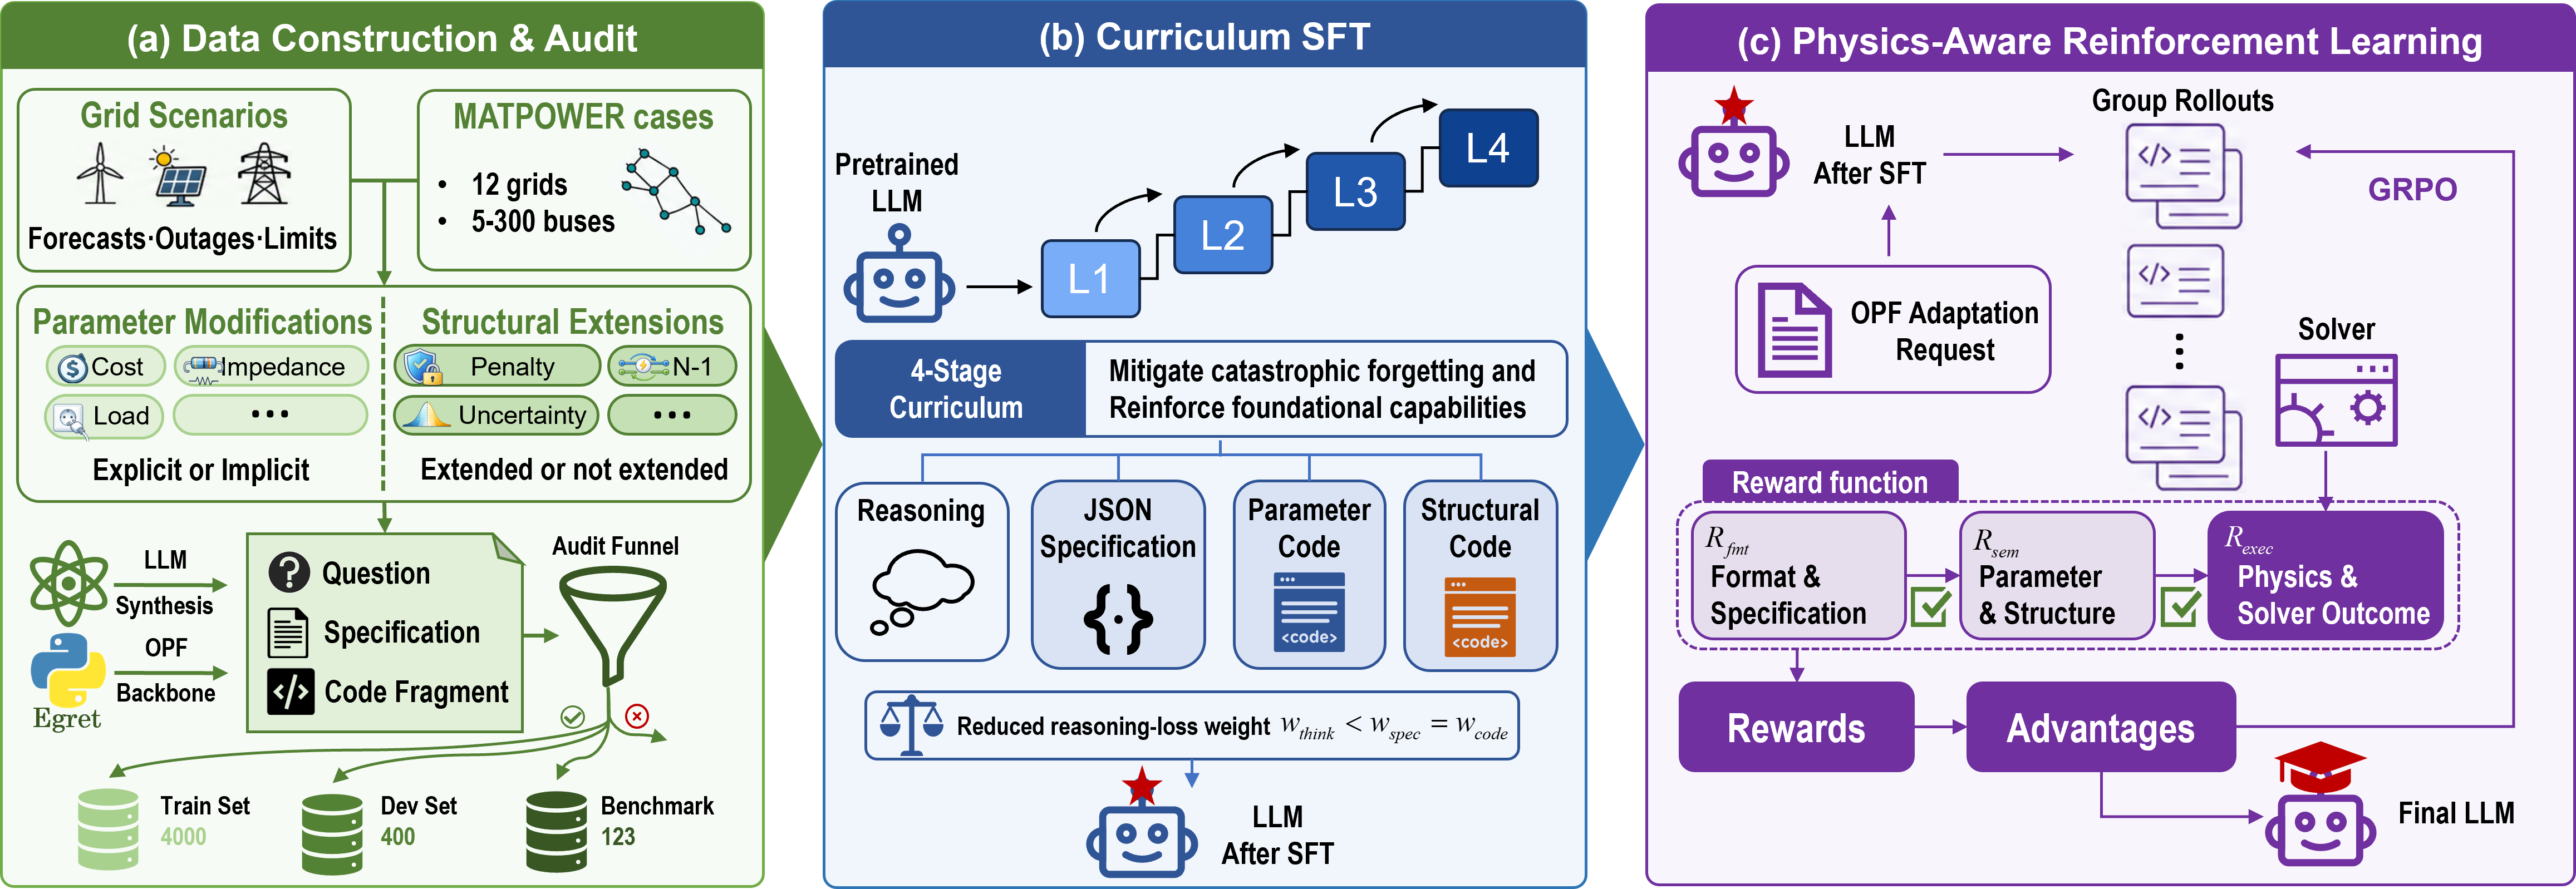
\includegraphics[width=\textwidth]{figures/framework.png}
\caption{Draft overview of the proposed workflow: audited construction of parameter-modification and structural-extension data, cumulative curriculum SFT, and physics-aware reinforcement learning with gated rewards and solver feedback.}
\label{fig:framework}
\end{figure*}

\subsection{Canonical OPF and Adaptation Operators}
Let $d$ collect the network data---loads, generator attributes, branch parameters, limits, costs, and status---and let $z$ collect the decision variables. A canonical AC or DC OPF backbone can be written abstractly as
\begin{subequations}\label{eq:base-opf}
\begin{align}
  \mathcal{Q}_{\mathrm{base}}(d):\quad
  \min_{z}\;&F_0(z;d) \label{eq:base-obj}\\
  \mathrm{s.t.}\;&H_0(z;d)=0, \label{eq:base-eq}\\
  &G_0(z;d)\le 0, \label{eq:base-ineq}
\end{align}
\end{subequations}
where $H_0$ contains the formulation-specific power-balance equations and $G_0$ contains operating bounds and network limits. Standard code for data loading, AC/DC model construction, and solver invocation is treated as trusted infrastructure.

An instruction $x$ may imply a parameter transformation $T_p$ and structural additions $(\Delta F,\Delta H,\Delta G)$. The intended adapted problem is
\begin{subequations}\label{eq:adapted-opf}
\begin{align}
  d' &= T_p(d;x),\\
  \min_z\;&F_0(z;d')+\Delta F(z;d',x)\\
  \mathrm{s.t.}\;&H_0(z;d')=0,\quad \Delta H(z;d',x)=0,\\
  &G_0(z;d')\le0,\quad \Delta G(z;d',x)\le0.
\end{align}
\end{subequations}
Examples of $T_p$ include changing a load forecast, derating a line, or taking a generator out of service. Examples of structural additions include reserve variables and headroom constraints, an emission cap, an N--1 security constraint family, or a voltage-deviation term in the objective.

\subsection{Difference-Based LLM Interface}
Rather than ask the LLM to regenerate~\eqref{eq:base-opf}, we define
\begin{equation}\label{eq:llm-interface}
(\hat{\mathcal S},\hat c_p,\hat c_s)=f_\theta(x),\qquad
\hat{\mathcal Q}=\operatorname{Assemble}(\mathcal{Q}_{\rm base};\hat c_p,\hat c_s),
\end{equation}
where $\hat{\mathcal S}$ is a JSON specification, $\hat c_p$ is a Python parameter hook applied to Egret's model data before construction, and $\hat c_s$ is a structural hook applied to the Pyomo model after construction. The structural hook contains \texttt{pass} when the base structure is retained. The answer contract contains four regions: a concise rationale, the JSON specification, the parameter hook, and the structural hook. The rationale is supervised with reduced weight and is not trusted as evidence of correctness.

The two insertion points provide both modularity and observability. Parameter code can be checked by comparing the complete post-modification data state with a trusted reference. Structural code can be checked after model assembly by inspecting objectives, variables, and constraints. Generated code is never allowed to replace the solver driver or the standard power-flow equations.

\subsection{Four-Level Task Hierarchy}
The task hierarchy crosses two axes: whether numerical changes are explicit or must be inferred from an operating scenario, and whether the canonical formulation is retained or extended. Table~\ref{tab:levels} summarizes the four combinations.

\begin{table}[!t]
\caption{Four-Level OPF Adaptation Hierarchy}
\label{tab:levels}
\centering
\footnotesize
\renewcommand{\arraystretch}{1.08}
\begin{tabular}{@{}clll@{}}
\toprule
Level & Parameter values & Structure & Representative demand \\
\midrule
L1 & Explicit & Retained & Direct data edit \\
L2 & Scenario-inferred & Retained & Infer object/direction \\
L3 & Explicit & Extended & Data edit plus model term \\
L4 & Scenario-inferred & Extended & Joint inference and extension \\
\bottomrule
\end{tabular}
\end{table}

L1 and L3 are evaluated with the values stated in the request. L2 and L4 contain two held-out runtime instantiations, labeled mild and severe, that are not exposed as numerical values in the question. Both instantiations must pass. This prevents a model from hard-coding one value while preserving the required direction and object identity.

\subsection{Verifiable Correctness}
Let $I_{\rm fmt}$ indicate a valid response contract, JSON schema, function signature, and Python syntax. Let $I_{\rm spec}$ indicate agreement of the case, formulation, grid objects, operations or directions, structural family, and solver requirements. Parameter correctness is defined by equality of the candidate and trusted post-states,
\begin{equation}
I_p=\mathbb{I}\!\left[T_{\hat c_p}(d;\xi)=T_{c_p^*}(d;\xi)\right],
\end{equation}
where $\xi$ is empty for explicit tasks and denotes a runtime strategy for inferred tasks. Structural correctness is
\begin{equation}
I_s=\mathbb{I}\!\left[\Phi(\hat{\mathcal Q})=\Phi(\mathcal Q^*)\right],
\end{equation}
where $\Phi$ is a semantic signature of the objective delta, added variables and constraints, and protected base-model components. In the current candidate evaluator, $I_{\rm solve}$ requires successful solver execution and reference-objective agreement. The final protocol will additionally record solver termination and explicit feasibility residuals. The strict end-to-end indicator is
\begin{equation}\label{eq:strict}
I_{\rm strict}=I_{\rm fmt}I_{\rm spec}I_pI_sI_{\rm solve}.
\end{equation}
This conjunction is deliberately stronger than code execution or objective agreement alone.

\section{Executable Dataset Construction}
\subsection{Python/Egret Backbone and Scope}
Egret is an open-source Python package built on Pyomo for electric-grid optimization~\cite{bynum2021egret,pyomoBook}; MATPOWER cases provide the public network instances~\cite{zimmerman2011matpower}. Egret's separation between model data and the algebraic Pyomo model naturally exposes the parameter and structural insertion points in~\eqref{eq:llm-interface}. The current scope includes continuous ACOPF and DCOPF adaptations. It does not cover unit commitment, transient simulation, protection logic, or autonomous online control.

The semantic release candidate uses 12 MATPOWER systems ranging from 5 to 300 buses: \texttt{case5}, \texttt{case6ww}, \texttt{case9}, \texttt{case14}, \texttt{case18}, \texttt{case24\_ieee\_rts}, \texttt{case30}, \texttt{case39}, \texttt{case57}, \texttt{case60nordic}, \texttt{case118}, and \texttt{case300}. Parameter changes cover active/reactive demand, voltage and generation limits, generation-cost coefficients, branch resistance/reactance/susceptance and ratings, transformer taps, and equipment status. Structural examples span the nine families listed in Table~\ref{tab:structures}. All L1/L2 records use ACOPF. In train and development data, each of L3 and L4 contains 425 ACOPF and 775 DCOPF records; the benchmark contains 11 ACOPF records in each structural level and 32 DCOPF records in total.

\begin{table}[!t]
\caption{Structural-Extension Coverage in Train and Development Data}
\label{tab:structures}
\centering
\footnotesize
\begin{tabular}{@{}lr@{}}
\toprule
Structural family & Examples \\
\midrule
Angle-difference penalty & 258 \\
Voltage-deviation penalty & 292 \\
Reactive-generation cost & 276 \\
N--1 contingency constraints & 266 \\
Spinning-reserve requirement & 246 \\
Regulation-up requirement & 254 \\
Quadratic-emission cost & 260 \\
CO$_2$ emission cap & 266 \\
Reactive-reserve requirement & 282 \\
\midrule
Total L3/L4 & 2400 \\
\bottomrule
\end{tabular}
\end{table}

\subsection{Synthesis and Benchmark Rebuilding}
We retain the task taxonomy and scenario concepts of ProOPF but do not mechanically translate ProOPF-D into Python. The original MATLAB corpus cannot directly supervise Egret/Pyomo APIs or provide the realized post-state and structural signatures required here. Training specifications and Python/Egret hooks are therefore synthesized and executed independently. The 123 benchmark questions are separately rebuilt from ProOPF-B scenarios, with corrections and revalidation where the Python interface or physical semantics differ from the original MATLAB implementation. All BP-v6 changes were fixed before evaluating any model trained on DP-v11. \drafttodo{Document the exact template/API/inherited-text provenance and quantify the ProOPF-B tasks retained, repaired, replaced, and added when the public release history is finalized.}

For each candidate task, the construction pipeline selects a real case and formulation, samples valid parameter targets and values or a scenario-direction pair, and optionally selects a structural family with its hyperparameters. A trusted parameter hook and structural hook are then assembled around the backbone. Explicit tasks are solved once; inferred tasks are solved under both runtime strategies. Only tasks that pass the applicable construction checks are retained. Natural-language questions describe the operating request without exposing internal level names, runtime placeholders, or held-out strategy values.

\subsection{Deterministic Audit Pipeline}
The pipeline is stricter than ``program runs and objective matches,'' but the construction-time and generated-answer checks have different coverage in V1.
\begin{enumerate}
  \item \emph{Interface and grid semantics}: required fields and hook syntax are validated; the case and AC/DC formulation must be valid; every target must resolve to the intended real bus, generator, load, or branch; and inactive quantities are excluded from incompatible formulations.
  \item \emph{Parameter post-state}: every retained hook is executed in a fresh subprocess, and the complete typed Egret \texttt{ModelData.data} tree is compared with the trusted post-state. This detects no-ops, wrong identifiers, wrong values, and collateral edits.
  \item \emph{Structural semantics}: trusted gold hooks are produced from controlled nine-family templates and paired with solved labels. For generated answers, candidate and trusted hooks are applied to separately constructed models; polynomial objective deltas and supported constraints are canonicalized so component names and term order do not affect equivalence. The verifier's nine positive families and targeted no-op, missing-term, wrong-coefficient, and base-tampering counterexamples pass regression tests. A full per-record structural re-audit of all 4523 gold records has not been claimed.
  \item \emph{Execution and objective}: benchmark gold programs must return an objective and match the reference within an absolute tolerance of $10^{-4}$ or relative tolerance of $10^{-3}$. Explicit termination-condition and feasibility-residual logging remain to be added to the final evaluator.
\end{enumerate}

The stated objective tolerance records the current software setting; it is not used as a substitute for semantic verification. \drafttodo{Before final evaluation, preregister the tolerance and report a tighter-tolerance sensitivity analysis.}

Hook execution uses a fresh subprocess with a timeout, and the caller handles serialized reports. This isolates parent-process Python state, but it is not an operating-system security sandbox: filesystem, network, and resource isolation remain deployment requirements.

Algorithm~\ref{alg:audit} summarizes the intended strict evaluation of one generated adaptation.

\begin{algorithm}[!t]
\caption{Strict Evaluation of One Generated OPF Adaptation}
\label{alg:audit}
\begin{algorithmic}[1]
\REQUIRE Request $x$, specification $\mathcal S$, hooks $(c_p,c_s)$, pristine case $d$
\STATE Parse response contract, $\mathcal S$, and Python AST
\STATE Resolve the case, formulation, and all grid objects
\FOR{each runtime strategy $\xi$ (one for explicit tasks, two for inferred tasks)}
  \STATE Run $c_p$ in a fresh subprocess and snapshot the post-state
  \STATE Compare the post-state with the trusted parameter oracle
  \STATE Build fresh candidate and trusted Egret/Pyomo models
  \STATE Run $c_s$ and compare semantic structural signatures
  \STATE Execute the assembled OPF and collect execution status and objective
  \STATE Reject if any required check fails
\ENDFOR
\RETURN Strict decision and per-gate report
\end{algorithmic}
\end{algorithm}

The audit exposed errors that objective-only filtering would miss. For example, CO$_2$ caps were originally expressed in MW but compared directly with per-unit generation variables. The corrected hook divides the cap by \texttt{baseMVA}; 266 records and 399 stored results were regenerated. Similarly, coefficient-based generator terms now store generator identifiers in addition to bus numbers, avoiding ambiguity when multiple generators share a bus.

\subsection{Source-Separated Split and Statistics}
Table~\ref{tab:data-split} reports the frozen candidate split. Development examples are sampled by semantic lineage: an explicit task and its inferred counterpart remain together, as do structurally retained and extended variants derived from the same source scenario. No lineage crosses train and development. The benchmark is separately rebuilt and has zero overlap with the training/development data under full-specification and parameter-identity signatures.

\begin{table}[!t]
\caption{Frozen Candidate Data Split}
\label{tab:data-split}
\centering
\footnotesize
\begin{tabular}{@{}lrrrrr@{}}
\toprule
Split & L1 & L2 & L3 & L4 & Total \\
\midrule
Train & 900 & 900 & 1100 & 1100 & 4000 \\
Development & 100 & 100 & 100 & 100 & 400 \\
Benchmark & 36 & 33 & 28 & 26 & 123 \\
\bottomrule
\end{tabular}
\end{table}

Across all single-level train, development, and benchmark records, 4523/4523 records pass the parameter-target and post-state audit, requiring 6782 hook executions. All 64 explicit benchmark gold programs solve and reproduce their stored objectives. All 59 inferred benchmark programs pass both strategies, for 118/118 successful strategy solves. The parameter/structural verifiers, strict evaluator, and data converter pass 34 targeted regression tests, including no-op, wrong-object, missing-constraint, wrong-coefficient, and base-model-tampering counterexamples. The benchmark covers six of the nine training structural families; emission-cost, emission-cap, and reactive-reserve extensions remain train/development-only and therefore cannot support test-set generalization claims in V1.

Two runtime strategies need not produce different objective values: this occurs in 202 L2 and 436 L4 train/development records and in 12 L2 and 9 L4 benchmark records, although their audited post-states differ. These records are retained because a nonbinding limit or unchanged active set can make the equality physically legitimate. They also provide direct evidence that objective-only evaluation cannot identify the intended modification and cannot support a monotonic ``mild versus severe'' claim by itself.

The remaining label decision concerns the auxiliary rationale: 49 train/development responses retain legacy mentions of the internal level taxonomy. User questions, prompts, and benchmark responses contain no such hints. \drafttodo{Before final retraining, either rewrite and fact-audit these rationales once or document their retention; do not change task identities, hooks, results, or splits.}

\section{Physics-Aware Post-Training}
\subsection{Cumulative Curriculum SFT}
The two hierarchy axes create a natural curriculum. Stage~1 learns the response contract and explicit data edits from L1. Stage~2 adds scenario-to-parameter inference through L2. Stage~3 introduces Pyomo structural construction through L3. Stage~4 combines scenario inference and structural extension through L4. Earlier data are retained in every later stage, yielding cumulative training sizes of 900, 1800, 2900, and 4000 and development sizes of 100, 200, 300, and 400. Replay is important because training only on a new level previously caused the model to invent structural extensions for simpler requests.

For a target response $y=(y_1,\ldots,y_T)$, SFT minimizes a token-weighted negative log likelihood,
\begin{equation}\label{eq:sft}
\mathcal L_{\rm SFT}(\theta)=-\sum_{t=1}^{T}w_t
\log p_\theta(y_t\mid x,y_{<t}),
\end{equation}
where specification and code tokens receive unit weight and rationale tokens receive $\lambda_{\rm r}<1$. The preliminary configuration uses $\lambda_{\rm r}=0.1$. This choice treats reasoning as soft guidance rather than a fixed template while concentrating supervision on the executable interface. \drafttodo{Confirm $\lambda_{\rm r}$ through an ablation on the frozen development set.}

\subsection{Three-Stage Physics-Aware Reward}
After SFT, reinforcement learning targets failures that token likelihood does not directly distinguish. For a sampled answer $y$, the proposed reward is
\begin{equation}\label{eq:reward}
R(y)=\alpha_f r_{\rm fmt}+g_1\alpha_s r_{\rm sem}
+g_1g_2\alpha_e r_{\rm exec},
\end{equation}
where $r_{\rm sem}$ is the realized grid/model-correctness stage, $g_1$ and $g_2$ indicate complete passage of the preceding gate, and $\alpha_f,\alpha_s,\alpha_e$ are stage weights.

The three rewards are defined as follows.
\begin{itemize}
  \item $r_{\rm fmt}$ checks the four response regions, JSON schema, required functions, and Python syntax. It provides inexpensive feedback before any generated code is executed.
  \item $r_{\rm sem}$ checks the case, AC/DC formulation, real grid objects, operations or directions, structural intent, parameter post-state, structural equivalence, and protected base-model invariants. It therefore evaluates the realized grid/model change rather than language semantics alone. The gold structural family, not a candidate-declared family, selects the verifier and prevents reward gaming through self-reported metadata.
  \item $r_{\rm exec}$ runs the complete adaptation and checks successful solver execution and reference-objective agreement. For L2/L4, both runtime strategies must pass. \drafttodo{Extend this stage with termination-condition and feasibility-residual checks before final RL.}
\end{itemize}

The gate ordering is intentional. A wrong-device edit cannot earn the solver reward merely because the resulting objective is close. A detached constraint cannot pass the semantic model check even if the unmodified backbone converges. Conversely, equivalent Pyomo expressions with different component names or term order can pass because verification operates on canonicalized model semantics rather than source-text equality.

\subsection{Shared Verification Infrastructure}
The object resolver, post-state comparator, structural verifier, and subprocess runner are currently used for auditing and strict candidate evaluation. The final RL reward is designed to call the same components rather than maintain a second definition of correctness. This makes error analysis directly actionable: if the SFT model primarily fails object identity, parameter post-state, or reserve construction on development data, the corresponding reward component can be emphasized without inspecting the held-out benchmark. \drafttodo{Wire the frozen verifier API into \texttt{RL/proopf\_reward.py} and add reward parity tests before running GRPO.}

\subsection{Group-Relative Policy Optimization}
The intended policy optimizer is group relative policy optimization (GRPO)~\cite{shao2024deepseekmath}. For each request $x$, the policy samples a group of $G$ completions with rewards $R_1,\ldots,R_G$. A normalized group advantage is
\begin{equation}
A_i=\frac{R_i-\operatorname{mean}(R_1,\ldots,R_G)}
{\operatorname{std}(R_1,\ldots,R_G)+\epsilon}.
\end{equation}
The clipped policy objective increases the likelihood of above-average verified adaptations while a KL term limits deviation from the SFT reference policy. The final reward weights, rollout count, KL coefficient, temperature, learning rate, and stopping rule must be selected only on the source-separated development set. Table~\ref{tab:rl-config} records the decisions that remain open in V1.

\begin{table}[!t]
\caption{RL Configuration to Be Finalized}
\label{tab:rl-config}
\centering
\footnotesize
\begin{tabular}{@{}ll@{}}
\toprule
Item & Draft setting \\
\midrule
Initialization & Best Stage-4 SFT checkpoint on dev \\
Policy optimizer & GRPO \\
Rollouts per request & \drafttodo{$G$} \\
Learning rate & \drafttodo{Select on dev} \\
Sampling temperature & \drafttodo{Select on dev} \\
KL coefficient & \drafttodo{Select on dev} \\
Reward weights & \drafttodo{$\alpha_f,\alpha_s,\alpha_e$} \\
Early stopping & Four-level dev macro strict accuracy \\
Test access & Once after configuration freeze \\
\bottomrule
\end{tabular}
\end{table}

\section{Experimental Protocol}
\subsection{Research Questions}
The final experiments are organized around five questions.
\begin{itemize}
  \item \textbf{RQ1}: Does domain SFT improve strict, executable OPF adaptation over the base model and a strong API model?
  \item \textbf{RQ2}: Does the cumulative curriculum retain earlier capabilities better than joint or non-replay training?
  \item \textbf{RQ3}: Which errors remain after SFT, and does Physics-Aware RL improve them without sacrificing simpler levels?
  \item \textbf{RQ4}: Which reward gates and deterministic verifiers are necessary to prevent no-op and objective-matching failures?
  \item \textbf{RQ5}: How does performance vary across AC/DC formulations, system sizes, modified object types, and structural families?
\end{itemize}

\subsection{Models, Training, and Decoding}
The preliminary SFT model starts from Qwen2.5-7B~\cite{qwen25}. It is full-parameter fine-tuned in bf16 with FSDP on four NVIDIA A100 GPUs, effective batch size 8, and reasoning-token weight 0.1. Each curriculum boundary restarts the optimizer and learning-rate scheduler. Table~\ref{tab:prelim-train} lists the completed pre-freeze run on ProOPF-DP-v10. The final paper must retrain on the source-separated \dataset{} split and select each checkpoint using its cumulative development set.

\begin{table}[!t]
\caption{Completed Preliminary SFT Configuration on DP-v10}
\label{tab:prelim-train}
\centering
\footnotesize
\setlength{\tabcolsep}{3.5pt}
\begin{tabular}{@{}lrrrr@{}}
\toprule
Stage & Train & Epochs & LR & Max tokens \\
\midrule
L1 & 1000 & 5 & $1.0\!\times\!10^{-5}$ & 2048 \\
L1+L2 & 2000 & 2 & $1.0\!\times\!10^{-5}$ & 2304 \\
L1+L2+L3 & 3200 & 2 & $7.5\!\times\!10^{-6}$ & 4096 \\
L1+L2+L3+L4 & 4400 & 2 & $5.0\!\times\!10^{-6}$ & 4096 \\
\bottomrule
\end{tabular}
\end{table}

Baselines include the unmodified Qwen2.5-7B and DeepSeek-V4-Flash. All models receive the same output contract and use greedy decoding for the reported preliminary comparison. ``Zero-demonstration'' means that the system prompt specifies the complete response schema but contains no worked answer; ``two-demonstration'' additionally includes two level-appropriate examples. This terminology avoids implying that the model receives no task instructions.

\drafttodo{For final experiments, record exact model revisions, tokenizer, PyTorch/Pyomo/Egret/solver versions, GPU hours, random seeds, decoding limits, API access date, and monetary cost. Add at least one current open-weight model and repeat the principal training setting across three seeds if resources permit.}

\subsection{Metrics}
The primary metric is the strict accuracy in~\eqref{eq:strict}. To diagnose failures, we also report the cumulative pass rates for parsing, semantic specification, parameter post-state, structural verification, execution, and objective agreement. Macro averages across L1--L4 prevent levels with more evaluation tasks from dominating model selection. All checkpoint, hyperparameter, and reward decisions use development data; \benchmark{} is reserved for final evaluation.

The preliminary results in Section~VII-A were produced before the deterministic semantic gates were integrated. Their historical ``strict E2E'' definition is only $I_{\rm fmt}I_{\rm run}I_{\rm obj}$ and must not be confused with~\eqref{eq:strict}. Its parser also permits limited tag/JSON normalization and fills selected metadata from the task context. These values are retained in this V1 draft to document the evidence already available, not as final frozen-benchmark claims.

\section{Results and Analysis}
\subsection{Preliminary Baseline and SFT Results}
Table~\ref{tab:prelim-results} reports the completed comparison on ProOPF-BP-v5. Under the legacy parse--execute--objective metric, the final SFT checkpoint improves Qwen2.5-7B from 0/123 to 15/123 in zero-demonstration evaluation and from 15/123 to 66/123 with two demonstrations. It equals the aggregate DeepSeek result with two demonstrations, although the level distribution differs: SFT is stronger on L2, whereas DeepSeek is stronger on L1, L3, and L4.

\begin{table*}[!t]
\caption{Preliminary Objective-Matching E2E Accuracy $E2E_{\rm obj}$ (\%) on ProOPF-BP-v5; These Values Must Be Rerun with the Finalized Strict Evaluator on BP-v6}
\label{tab:prelim-results}
\centering
\footnotesize
\begin{tabular}{@{}llrrrrr@{}}
\toprule
Prompt & Model & L1 & L2 & L3 & L4 & All \\
\midrule
Two demonstrations & Qwen2.5-7B base & 30.56 & 12.12 & 0.00 & 0.00 & 12.20 \\
& DeepSeek-V4-Flash & \textbf{97.22} & 24.24 & \textbf{50.00} & \textbf{34.62} & \textbf{53.66} \\
& Qwen2.5-7B + SFT & 80.56 & \textbf{66.67} & 35.71 & 19.23 & \textbf{53.66} \\
\midrule
Zero demonstration & Qwen2.5-7B base & 0.00 & 0.00 & 0.00 & 0.00 & 0.00 \\
& DeepSeek-V4-Flash & 0.00 & 0.00 & 0.00 & 0.00 & 0.00 \\
& Qwen2.5-7B + SFT & \textbf{5.56} & \textbf{24.24} & \textbf{14.29} & \textbf{3.85} & \textbf{12.20} \\
\bottomrule
\end{tabular}
\end{table*}

The pass-rate funnel in Table~\ref{tab:prelim-funnel} clarifies the zero-demonstration zeros. DeepSeek produces a parseable response for 91/123 tasks but no executable Egret adaptation. The base Qwen model executes only 2/123 responses and none reaches the objective. Thus, the result reflects an interface and implementation mismatch, not an absence of all OPF reasoning. With demonstrations, both strong API prompting and SFT greatly improve execution.

\begin{table}[!t]
\caption{Preliminary Aggregate Response Funnel (Counts out of 123)}
\label{tab:prelim-funnel}
\centering
\footnotesize
\setlength{\tabcolsep}{3pt}
\begin{tabular}{@{}llrrr@{}}
\toprule
Prompt & Model & Parse & Execute & $E2E_{\rm obj}$ \\
\midrule
Zero & Qwen base & 64 & 2 & 0 \\
& DeepSeek-V4 & 91 & 0 & 0 \\
& Qwen + SFT & 66 & 24 & 15 \\
\midrule
Two-demo & Qwen base & 66 & 23 & 15 \\
& DeepSeek-V4 & 123 & 66 & 66 \\
& Qwen + SFT & 109 & 79 & 66 \\
\bottomrule
\end{tabular}
\end{table}

The hardest setting is L4, where the model must infer parameter direction and generate a structural extension. L4 two-demonstration parsing reaches 22/26 for the SFT checkpoint, but only 7/26 execute and 5/26 match the objective. This gap motivates semantic and structural reward components rather than further format-only training.

\subsection{Curriculum Retention and Residual Errors}
Within the preliminary run, the L3 specialist solves 16/28 L3 two-demonstration tasks under the legacy E2E metric, whereas the final Stage-4 checkpoint solves 10/28. L1 and L2 improve after later stages, but interference between explicit and inferred structural extensions remains. The final experiment will compare cumulative curriculum, one-stage mixed SFT, and curriculum without replay on the same fixed development and test sets.

The pre-freeze error analysis records 100 JSON parse failures among 440 generated answers, 43 Python syntax errors, and 78 failures in implicit runtime-identity mapping. After parsing succeeds, frequent semantic failures include adjacent but incorrect component identifiers, confusion between load and bus indices, unsupported Egret/Pyomo fields, missing structural terms, and structurally valid but numerically incorrect objectives. These categories map directly to the three reward gates.

\subsection{Preliminary RL Evidence}
An early L1 prototype contains one archived 36-task few-shot run with 22/36 objective-correct outputs, compared with 13/36 for its preceding SFT checkpoint. A second appended run reached 20/36, and neither run used the current strict protocol. They predate the frozen data, source-separated development set, three-stage deterministic verifier, and current four-level SFT. Moreover, the archived L3 artifacts do not reproduce the improvement cited in earlier digest drafts. Consequently, this paper makes no RL performance claim from those runs and does not compare them with Table~\ref{tab:prelim-results}.

\drafttodo{Run GRPO from the development-selected \dataset{} SFT checkpoint; report L1--L4 zero-/two-demonstration strict accuracy, component rewards, KL, response length, solver-call rate, wall time, and three-seed uncertainty.}

\subsection{Required Ablations and Final Result Table}
Table~\ref{tab:final-placeholder} defines the minimum final comparison. Each dash is an intentionally missing experiment, not a zero. The accompanying ablations will compare joint versus curriculum SFT, replay versus no replay, rationale weight 1.0 versus 0.1, objective-only versus gated reward, removal of the semantic gate, removal of the structural verifier, and removal of solver feedback.

\begin{table}[!t]
\caption{Final Strict Accuracy on \benchmark{} (Experiment Placeholder)}
\label{tab:final-placeholder}
\centering
\scriptsize
\setlength{\tabcolsep}{2.2pt}
\begin{tabular}{@{}lrrrrr@{}}
\toprule
Model/Training & L1 & L2 & L3 & L4 & Macro \\
\midrule
\multicolumn{6}{@{}l}{\emph{Zero demonstration}} \\
Qwen2.5-7B base & -- & -- & -- & -- & -- \\
Current open-weight baseline & -- & -- & -- & -- & -- \\
Qwen2.5-7B + SFT & -- & -- & -- & -- & -- \\
Qwen2.5-7B + SFT + RL & -- & -- & -- & -- & -- \\
\midrule
\multicolumn{6}{@{}l}{\emph{Two demonstrations}} \\
Qwen2.5-7B base & -- & -- & -- & -- & -- \\
Strong API baseline & -- & -- & -- & -- & -- \\
Qwen2.5-7B + SFT & -- & -- & -- & -- & -- \\
Qwen2.5-7B + SFT + RL & -- & -- & -- & -- & -- \\
\bottomrule
\end{tabular}
\end{table}

\subsection{Planned Engineering Case Studies}
The final paper will include two traceable cases. The first will show a parameter-only request and report the resolved object, before/after data values, and AC/DC objective. The second will combine parameter changes with a reserve, emission, or N--1 structural extension and report the added Pyomo components and, after the evaluator extension is complete, feasibility residuals. Each case will compare the base model, SFT, and SFT+RL outputs at every verifier gate. This presentation is intended to connect aggregate code-generation accuracy to the actual power-system model being solved.

\section{Discussion}
\subsection{Why Adaptation Rather Than Full Generation?}
The fixed-backbone design is not merely a device for shortening the target sequence. It encodes an engineering boundary: standard power-flow equations, data loading, and solver control remain in reviewed software, while the model generates only the changing portion. This reduces duplicated code, makes every generated operation inspectable, and allows the verifier to attribute an error to a parameter or structural hook. Full generation may remain necessary for genuinely new formulations, but it expands both the learning problem and the safety surface.

\subsection{Operational Interpretation}
The present system should be viewed as an offline or human-supervised modeling assistant. A planner or operator supplies a study requirement, the LLM proposes a model difference, deterministic gates reconstruct and solve the candidate, and a human can inspect the compact change and audit report. The current evidence does not justify autonomous real-time dispatch, automatic protection actions, or direct execution against a production energy-management system.

The parameter--structure abstraction nevertheless has an operational basis. Forecast and availability changes naturally map to data updates; reserve, emissions, contingency, and corrective requirements map to additions in the objective or constraint set. Future evaluation should measure not only code correctness but also whether the adapted model represents the intended outage, reserve margin, security limit, or policy requirement and whether it changes the resulting dispatch in the expected physical direction.

\subsection{Safety and Deployment Boundaries}
Generated Python is untrusted. It must run in an isolated process with explicit imports, time and resource limits, a read-only case library, and no network or credential access. Passing a deterministic verifier is necessary but not sufficient for deployment: the verifier covers only its supported task and structural families. Unsupported requests should abstain or be routed to expert review rather than forced into the nearest known template.

Inference-time repair is complementary to post-training. A repair system can diagnose residual failures after the proposed model generates a candidate. Conversely, a better trained generator reduces the number and severity of repairs. A controlled comparison should distinguish first-pass accuracy, repair success, additional solver calls, and preservation of initially correct outputs.

\subsection{Limitations and Threats to Validity}
First, the 12 public systems and nine training structural families do not cover the diversity of utility models, and the final benchmark contains only six systems and six structural families. Second, the benchmark focuses on continuous AC/DC OPF; unit commitment, stochastic and robust optimization, transient security, and sequential switching remain outside scope. Third, reference-hook comparison assumes that audited gold implementations are correct, although the multi-stage audits reduce this risk. Fourth, preliminary scores were produced on the pre-freeze dataset, a legacy metric, and a permissive parser/executor that must be replaced by the frozen protocol. Fifth, a single 7B base model cannot establish architecture- or scale-independent conclusions. Finally, solver convergence and objective agreement can still mask requirements not encoded in the specification, which motivates future human review and scenario-level validation.

\section{Conclusion}
This paper operationalizes language-driven OPF programming as a small, auditable adaptation around a trusted Python/Egret backbone. The task representation separates parameter updates from structural extensions and exposes both for deterministic verification. A source-separated four-level corpus and cumulative curriculum SFT address capability acquisition; the proposed gated Physics-Aware reward is designed to align subsequent RL with interface, realized grid/model, and solver correctness. Existing preliminary results show that domain SFT can substantially improve executable generation, while complex structural adaptation remains the principal bottleneck. \drafttodo{Replace the final empirical claim after completing the frozen SFT, RL, ablation, and case-study experiments.}

\section*{Acknowledgment}
\drafttodo{Add funding, data/code availability, and acknowledgments after the author team confirms them.}

\bibliographystyle{IEEEtran}
\bibliography{references}

\end{document}
